In the following section, we perform a number of numerical experiments to
validate the accuracy and complexity of our method. We close with an application
to computing Fourier transforms of radial kernel functions from statistics.

\subsection{Comparison to direct evaluation}

We start by empirically verifying the analysis in Theorem~\ref{thm:complexity}.
In order to study the impact of each of the relevant parameters independently,
we take $n$ equispaced points $r_k$ in the interval $[0,\sqrt{10^5}]$ and $m$
equispaced frequencies $\omega_j$ in the interval $[0,p/\sqrt{10^5}]$. First, we
fix $m=10^3$ and $p=10^5$ while increasing $n$. Next, we fix $n=10^3$ and
$p=10^5$, this time increasing $m$. Finally, we fix both $n = m = 10^3$ while
increasing $p$. Figure~\ref{fig:nmp-scaling} shows the CPU time for the NUFHT as
well as for direct summation in each of these scenarios. We observe the linear
or quasilinear scaling expected from Theorem~\ref{thm:complexity} with each of
$n, m,$ and $p$. Note in particular that the NUFHT scales with $p$ while direct
summation does not. Therefore, if a DHT is desired with relatively few points
with a very large space-frequency product, direct summation may give superior
performance, although such circumstances are rare in practice.

Next, we study the more typical scenario where the space-frequency product $p$
grows linearly with $n$, as discussed in Corollary~\ref{cor:complexity}. Here we
study two cases. First, we consider the Fourier-Bessel expansion where $\omega_j
= \mathrm{j}_{\nu, j}$ and $r_k = \mathrm{j}_{\nu, k}/\mathrm{j}_{\nu, n+1}$
with $n = m$. This is the direct analogue of the discrete Fourier transform as
the points and frequencies are the scaled roots of the basis, and the resulting
points and frequencies are quasi-equispaced for small to moderate $\nu$. 

We also consider the case of exponentially distributed points and frequencies
$\omega_j = r_j = 10^{\log_{10}(j) - \log_{10}(n)/2}$ with $n = m$. This is a
somewhat pathological worst case scenario for our algorithm, as the simple
calculation
\begin{equation}
  \sqrt{\frac{\Omega z}{R}} = \argmax_{\frac{z}{R} \leq \omega \leq \Omega} \ (\Omega - \omega)\left(R - \frac{z}{\omega}\right)
\end{equation}
shows that if we subdivide a block with space frequency product $\Omega R$ at a
point $(\omega, r)$ which lies on the curve $\omega r = z$, then the largest
possible space-frequency product $p$ for the resulting lower right asymptotic
block is achieved by taking $\omega$ to be the mid-point of $[\frac{z}{R},
\Omega]$ on a log scale. In other words, points and frequencies which are
exponentially distributed result in the highest possible space-frequency product
$p$ for every asymptotic block at every level. From
Theorem~\ref{thm:complexity}, maximizing $p$ drives the cost of the NUFHT. This
distribution of points and frequencies is also challenging because it leads to
equally-sized square blocks at every level, which guarantees that all blocks are
subdivided the maximum number of times before yielding sufficiently small direct
blocks.

Figure~\ref{fig:both-scaling} shows the CPU time needed to evaluate the NUFHT in
the Fourier-Bessel and exponentially-distributed cases with $\nu=0$ and
$\epsilon=10^{-8}$. Both cases eventually demonstrate the expected $\bO(n\log
n)$ scaling. As a result of to the challenges just discussed for the
exponentially-distributed case, its runtime is up to an order of magnitude
slower than the Fourier-Bessel series.

Next, we study the impact of the order $\nu$ and tolerance $\epsilon$ on the
runtime. As $\nu$ increases or $\epsilon$ decreases, the number of necessary
terms $L$ and $M$ in the local and asymptotic expansions respectively both grow.
From Theorem~\ref{thm:complexity}, we expect the runtime to grow linearly with
$L + M$. Figure~\ref{fig:both-scaling} shows the runtime of our method for
various $\epsilon$ with $\nu=0$ held constant, as well as for multiple $\nu$
with $\epsilon=10^{-8}$ fixed. The scaling of the algorithm is similar in all
cases, while the prefactors vary --- a transform with $\epsilon = 10^{-15}$ is
about an order of magnitude slower than using $\epsilon = 10^{-4}$, and an order
100 transform is almost two orders of magnitude slower the order-0 equivalent.

Finally, we study the relative error in the output $\vct{g}$ as a function of
the desired tolerance $\epsilon$. To do this, we fix $n$ and form a sparse
vector $\vct{f} \in \R^n$ with 1000 nonzero entries whose indices are selected
at random and whose values are independent standard Gaussian. We evaluate the
Fourier-Bessel series using the NUFHT with the full vector $\vct{f}$ as input,
and denote the output as $\vct{\tilde{g}}$. We then use direct summation on only
the nonzero entries to generate a reference result $\vct{g}$ which is
computationally tractable. Figure~\ref{fig:accuracy} shows the 2-norm relative
error $\norm[2]{\vct{g} - \vct{\tilde{g}}} / \norm[2]{\vct{g}}$ between the
NUFHT and the reference. For small transforms with $n=10^3$, the relative error
demonstrates excellent agreement with the tolerance $\epsilon$ down to $\epsilon
= 10^{-13}$ or so. This suggests that the analysis used in
Section~\ref{sec:approx} to determine the necessary number of local and
asymptotic terms is fairly tight. For larger transforms, however, the error
saturates, and regardless of the tolerance $\epsilon$ our method gives at most 9
digits of accuracy for transforms of size $n=10^7$. This is a well-known
limitation of existing NUFFT methods, for which the error generally scales like
$n$ times machine precision \cite[Remark 9]{barnett2019parallel}.

\begin{figure}
  \centering
  \newcommand\twa{0.29cm} \newcommand\tw{0.43cm}
  \begin{subfigure}[b]{0.32\textwidth}
    \begin{tikzpicture}
        \draw (0, 0) node[inner sep=0] {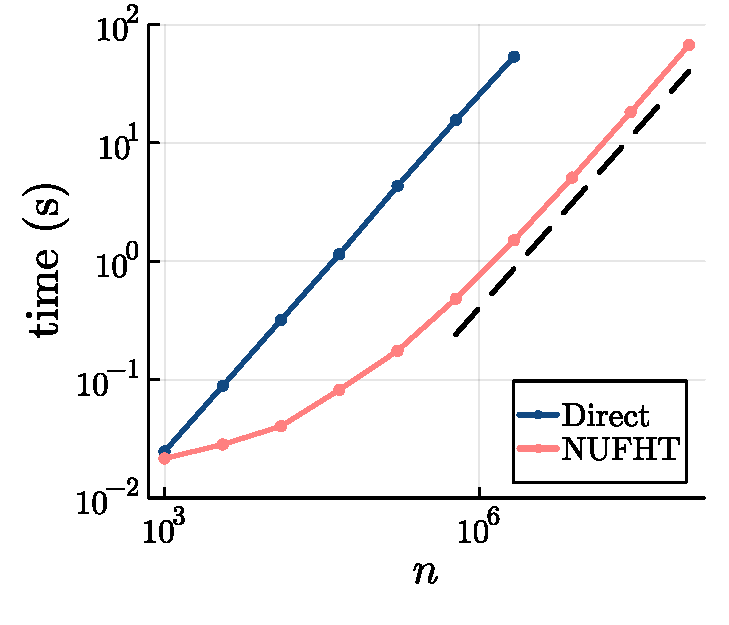
\includegraphics[height=0.92\textwidth,
        trim={0.4cm 0 0.5cm 0}, clip]{./figures/n_scaling.pdf}}; \draw (1.5,
        0.3) node {\small $\bO(n)$};
    \end{tikzpicture}
  \end{subfigure}
  \hfill
  \begin{subfigure}[b]{0.32\textwidth}
    \begin{tikzpicture}
        \draw (0, 0) node[inner sep=0] {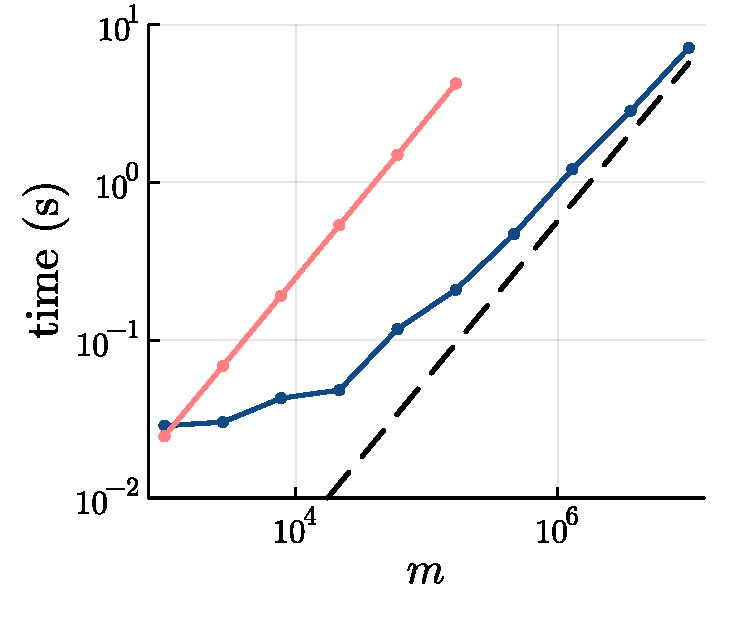
\includegraphics[height=0.92\textwidth,
        trim={1.3cm 0 0.5cm 0}, clip]{./figures/m_scaling.pdf}}; \draw (1.3,
        0.3) node {\small $\bO(m)$};
    \end{tikzpicture}
  \end{subfigure}
  % \hfill 
  \begin{subfigure}[b]{0.32\textwidth}
    \begin{tikzpicture}
        \draw (0, 0) node[inner sep=0] {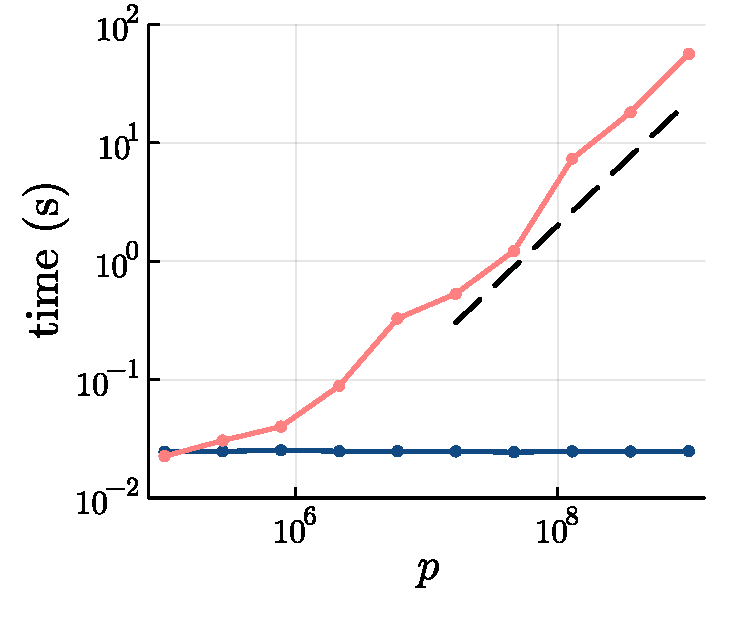
\includegraphics[height=0.92\textwidth,
        trim={1.3cm 0 0.5cm 0}, clip]{./figures/p_scaling.pdf}}; \draw (1.45,
        0.1) node {\small $\bO(p\log p)$};
    \end{tikzpicture}
  \end{subfigure}
  \caption{Scaling with $n$, $m$, and $p$ respectively, with the other variables held constant. In the first two plots, $p=10^5$ and $m$}
  \label{fig:nmp-scaling}
\end{figure}

\begin{figure}
  \centering
  \begin{subfigure}[b]{0.32\textwidth}
    \begin{tikzpicture} 
        \draw (0, 0) node[inner sep=0] {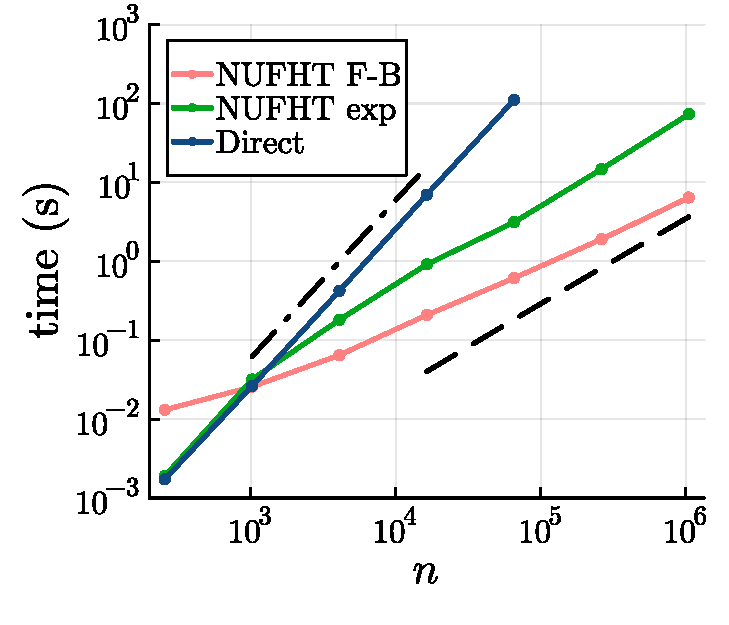
\includegraphics[height=0.92\textwidth,
        trim={0.4cm 0 0.5cm 0}, clip]{./figures/both_scaling.pdf}}; \draw (1.25,
        -0.5) node {\small $\bO(n\log n)$}; \draw (-0.7, 0.4) node {\small
        $\bO\big(n^2\big)$};
    \end{tikzpicture}
  \end{subfigure}
  \hfill
  \begin{subfigure}[b]{0.32\textwidth}
    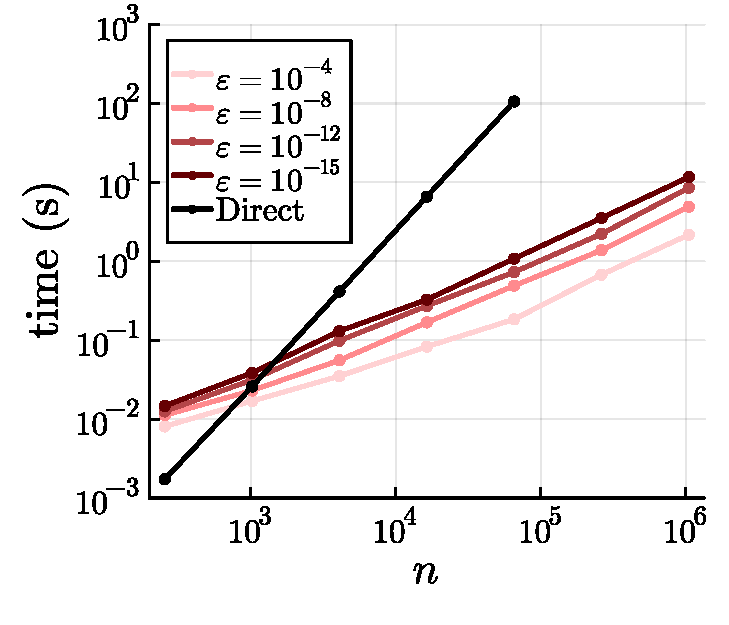
\includegraphics[height=0.92\textwidth, trim={1.3cm 0 0.5cm 0}, clip]{./figures/tol_scaling.pdf}
  \end{subfigure} 
  % \hfill 
  \begin{subfigure}[b]{0.32\textwidth}
    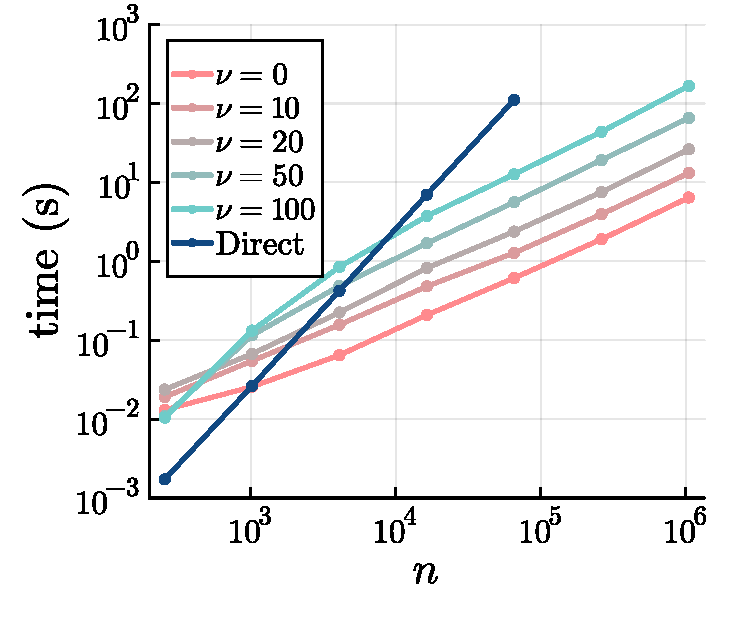
\includegraphics[height=0.92\textwidth, trim={1.3cm 0 0.5cm 0}, clip]{./figures/nu_scaling.pdf}
  \end{subfigure}
  \caption{Scaling with $n$ for $p = \bO(n)$ test cases. In the first plot, we
  fix $\nu = 0, \epsilon = 10^{-8}$ and time the NUFHT for both the
  Fourier-Bessel and exponentially distributed cases. In the second and third
  plots, we consider the Fourier-Bessel series only, and fix one of the
  parameters $\nu = 0$ and $\epsilon = 10^{-8}$ while varying the other. The
  timings of direct summation and Fourier-Bessel series from the first plot are
  repeated in the other two plots for reference.}
  \label{fig:both-scaling}
\end{figure}

\begin{figure}
  \centering
  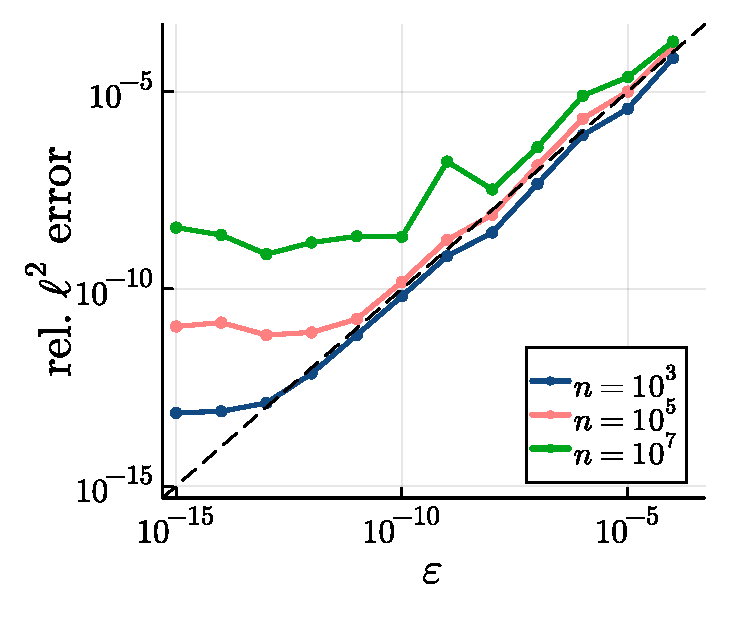
\includegraphics[width=0.4\textwidth]{./figures/accuracy.pdf}
  \caption{Relative 2-norm error $\norm[2]{\vct{g} - \vct{\tilde{g}}} /
  \norm[2]{\vct{g}}$ as a function of tolerance $\epsilon$ for a DHT of order
  $0$ for various $n$.}
  \label{fig:accuracy}
\end{figure}

\subsection{Computing Fourier transforms of radial functions}

For radial functions $f(\bm{r}) = f(\norm{\bm{r}})$ in $\R^d$, one can integrate
out the radial variables analytically, reducing the $d$-dimensional Fourier
integral to a single Hankel transform
\begin{align} \label{eq:radial-fourier}
    \hat{f}(\bm{\omega}) 
    = \int_{\R^d} f(\norm{\bm{r}}) e^{i\bm{\omega}^\top \bm{r}} \dif{\bm{r}}
    = \frac{(2\pi)^{\frac{d}{2}}}{\omega^{\frac{d}{2} - 1}} \int_0^\infty f(r) J_{\frac{d}{2} - 1}(\omega r) r^{\frac{d}{2}} \dif{r}.
\end{align}

We compare two methods of computing $\hat{f}$ for the indicator function of the
unit disk $f(r) = \ind{0 \leq r \leq 1}$ to absolute error $\epsilon = 10^{-12}$
at $n$ equispaced points $\omega_j \in [0, \omega_{\text{max}}]$. First, we use
a Gauss-Legendre quadrature rule on $[0,1]$ with nodes $r_k$ and weights $w_k$.
We utilize the NUFHT to compute the resulting sum
\begin{align}
  \hat{f}(\omega) 
  &= 2\pi\int_0^1 f(r) J_0(\omega r) r \dif{r} \\
  &\approx 2\pi \sum_{k=1}^m w_k f(r_k) J_0(\omega r_k) r_k,
\end{align}
doubling the number of nodes $m$ until the error in the computed integral is
less than $\epsilon$. Second, we build a two-dimensional quadrature rule in
polar coordinates, using the same $m$-point Gauss-Legendre rule in $r$ and a
$t_k$-node trapezoidal rule in $\theta$ on each circle of radius $r_k$. We
double the number of trapezoidal nodes $t_k$ in each circle until the error in
the corresponding radial integral is less than $\epsilon$. We then utilize the
2D NUFFT to compute the resulting double sum
\begin{align}
  \hat{f}(\omega) 
  &= \frac{1}{4\pi^2} \int_0^{2\pi} \int_0^1 f(r) e^{-i\omega r\cos\theta} r \dif{r} \dif{\theta} \\
  &\approx \frac{1}{4\pi^2} \sum_{k=1}^{m} w_k r_k f(r_k) \frac{2\pi}{t_k} \sum_{s=1}^{t_k} \exp\left\{-i\omega r_k\cos\left(\frac{2\pi s}{t_k}\right)\right\}.
\end{align}

If only low frequencies $\omega$ are desired, e.g. $\omega_{\text{max}} = 64$,
the integrands are only mildly oscillatory and few trapezoidal nodes are
required. In combination with the relative ease of amortizing costs in the
NUFFT, the two-dimensional transform is often faster than the NUFHT. However,
for larger $\omega_{\text{max}}$ the integrands become more oscillatory, and in
two dimensions $m = \bO(\omega_{\text{max}}^2)$ nodes are needed to resolve
these oscillations. Therefore the $\bO(m)$ spreading step in the NUFFT becomes
prohibitively expensive. However, by using radial symmetry to reduce to a
one-dimensional integral, the NUFHT requires only $\bO(\omega_{\text{max}})$
quadrature nodes, avoiding the curse of dimensionality.
Figure~\ref{fig:fourier-test} shows an example quadrature and runtimes for both
the NUFFT and NUFHT approaches. Note that for $\omega_{\text{max}} = 2^{15}$ the
2D NUFFT is orders of magnitude slower than the NUFHT for most $n$, and for even
larger $\omega_{\text{max}}$ the quadratic scaling of the 2D NUFFT with frequency
makes the computation intractable on a laptop, while the NUFHT's linear scaling
with frequency allows evaluation of the Fourier transform at much higher frequencies
at an only moderately increasing cost.

\begin{figure}
  \centering
  \begin{subfigure}[b]{0.38\textwidth}
    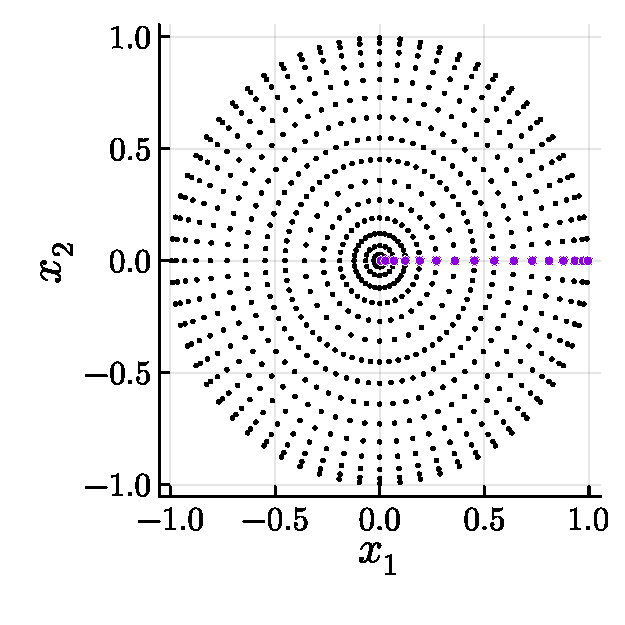
\includegraphics[height=\textwidth]{./figures/quadrature_2D.pdf}
  \end{subfigure}
  % \hfill
  \begin{subfigure}[b]{0.60\textwidth}
    \begin{tikzpicture} 
      \draw (0, 0) node[inner sep=0]
      {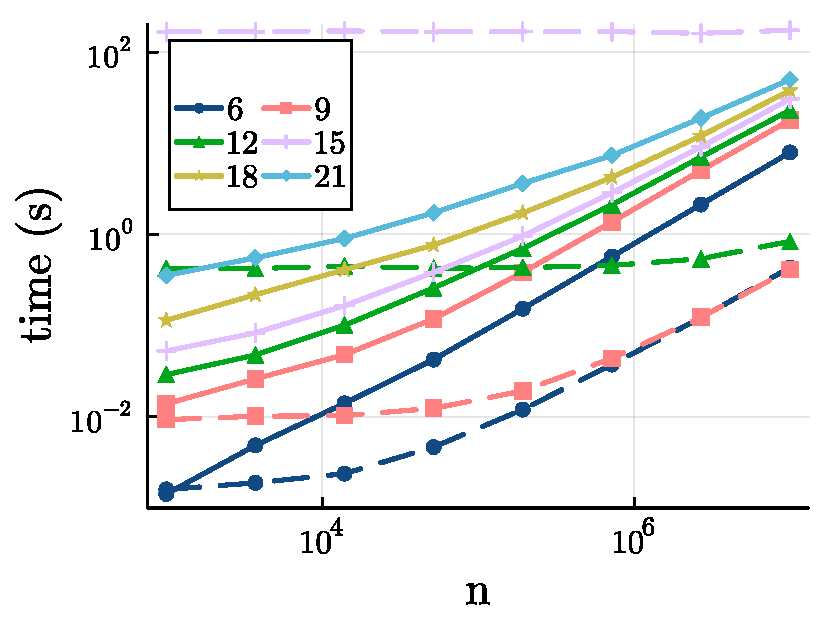
\includegraphics[height=0.63\textwidth]{./figures/fourier_scaling.pdf}};
      \draw (-1.2, 1.92) node {\scriptsize $\log_2\omega_{\text{max}}$};
    \end{tikzpicture}
  \end{subfigure}
  \caption{Example two-dimensional quadrature nodes for the NUFFT, with
  one-dimensional radial Gauss-Legendre quadrature on $[0,1]$ for the NUFHT
  emphasized. Runtime comparison between NUFHT and 2D NUFFT for various choices
  of the maximum frequency $\omega_{\text{max}}$ and the number of  evaluation
  points $n$. Solid lines indicate the NUFHT, and the corresponding dashed lines
  indicate the 2D NUFFT.}
  \label{fig:fourier-test}
\end{figure}

% \subsubsection{Higher dimensions}

% Using spherical Bessel function identities \cite[10.47.3,
% 10.49.2]{olver2010nist}, one can see that for half-integer $\nu$, Hankel's
% expansion (\ref{eq:asymptotic-expansion}) is no longer just an asymptotic
% expansion, but an exact formula. % \begin{align} J_{\frac{d}{2}-1}(z) &=
% \sqrt{\frac{2z}{\pi}} %   j_{\frac{d-3}{2}}(z) \\
% %   &= \sqrt{\frac{2}{\pi z}} \left( \cos\left(\mu\right) \sum_{\ell=0}^{M-1}
% %     (-1)^\ell \frac{a_{2\ell}\left(\frac{d}{2}-1\right)}{z^{2\ell}} - %
% \sin\left(\mu\right) \sum_{\ell=0}^{M-1} (-1)^\ell %
% \frac{a_{2\ell+1}\left(\frac{d}{2}-1\right)}{z^{2\ell+1}} \right) %
% \end{align} where $\mu := z - \frac{(2\nu+1)\pi}{4}$. For example, the kernel
% of the integral transform in (\ref{eq:radial-fourier}) for $d = 3$ is
% \begin{align} J_{\frac{1}{2}}(z) = \sqrt{\frac{2}{\pi z}} \sin(z), \end{align}
% and the corresponding NUFHT can be evaluated using a single NUFFT.

% The curse of dimensionality demonstrated in the two-dimensional case only
% intensifies in higher dimensions, for which the requirement of $\bO(m^d)$
% quadrature nodes is infeasible for even small $m$. In contrast, the NUFHT only
% ever requires one-dimensional quadrature, and is relatively robust to the
% distribution of $\omega_j$ and $r_k$, and to dimension for $d \leq 20$ or so.
% In even higher dimensions $d > 20$, the number of terms in the Hankel and Wimp
% expansions needed to maintain accurate evaluation increases, and the methods
% presented here become inefficient in practice, despite retaining their
% quasilinear asymptotic complexity. There exist several alternative asymptotic
% expansions in this large $\nu$ regime which can be leveraged for fast
% evaluation of $J_\nu(z)$~\cite{heitman2015asymptotics, olver2010nist}.
% %\cite[10.19]{heitman2015asymptotics, olver2010nist} However, the terms in
% these asymptotics are not sinusoids which can be efficiently evaluated with
% the NUFFT, and thus turning them into an analysis-based fast transform remains
% an open problem.

\subsection{Fourier-Bessel expansions}

Finally, we demonstrate the application of the nonuniform Hankel transform to
partial differential equations through the Fourier-Bessel expansion. The bessel
functions $J_m$ appear naturally as the radial components of separation of
variables solutions to the wave equation and Helmholtz equation with homogenous
Dirichlet boundary conditions.

First, expand $f$ into a Fourier series on the circle of radius $r$
\begin{align}
  f(r, \theta) 
  &\ = \sum_{\ell=-\infty}^\infty \alpha_\ell(r) e^{i\ell\theta}, \qquad
  \alpha_\ell(r) 
  := \int_0^{2\pi} f(r, \theta) e^{-i\ell\theta} \dif{\theta},
\end{align}
then expand each $\alpha_\ell$ into a Fourier-Bessel series
\begin{align}
  \alpha_\ell(r) 
  &\ = \sum_{j=0}^\infty \beta_{j\ell} J_\nu(\mathrm{j}_{\nu,j}r), \qquad
  \beta_{j\ell} := \frac{2}{J_{\nu+1}(\mathrm{j}_{\nu,j})^2} \int_0^1 \alpha_\ell(r) J_\nu(\mathrm{j}_{\nu,j}r) \, r \dif{r}.
\end{align}
This leads to the Fourier-Bessel series of order $\nu$ for $f$ on the disk
\begin{align}
  f(r, \theta) 
  &= \sum_{\ell=-\infty}^\infty \sum_{j=0}^\infty \beta_{j\ell} J_\nu(\mathrm{j}_{\nu,j}r) e^{i\ell\theta}.
\end{align}